\documentclass[11pt]{article}
\usepackage[margin=1in]{geometry}
\usepackage[T1]{fontenc}
\usepackage{lmodern}
\usepackage{amsmath,amssymb,amsthm,mathtools}
\usepackage{booktabs,array}
\usepackage{xcolor}
\usepackage{tikz}
\usetikzlibrary{arrows.meta,positioning,calc,fit,backgrounds,decorations.pathmorphing,shapes.geometric}
\usepackage[colorlinks=true,linkcolor=blue!55!black,citecolor=blue!55!black,urlcolor=blue!55!black]{hyperref}
\usepackage{enumitem}
\usepackage{microtype}
\usepackage{caption}

\definecolor{slate}{HTML}{263445}
\definecolor{bluefill}{HTML}{DCEAF4}
\definecolor{tealfill}{HTML}{D9EEE8}
\definecolor{amberfill}{HTML}{F7E9C8}
\definecolor{rosefill}{HTML}{F3DCDC}
\definecolor{muted}{HTML}{5C6875}

\newtheorem{definition}{Definition}[section]
\newtheorem{proposition}[definition]{Proposition}
\newtheorem{remark}[definition]{Remark}
\newtheorem{principle}[definition]{Design principle}
\newcommand{\supp}{\operatorname{supp}}
\newcommand{\TV}{\operatorname{TV}}
\newcommand{\Sh}{\mathcal{Sh}}
\newcommand{\Ctx}{\mathcal{C}}
\newcommand{\Amb}{\mathcal{A}}
\newcommand{\Prob}{\mathcal{P}}
\newcommand{\Ob}{\mathfrak{O}}
\newcommand{\slack}{\operatorname{slack}}
\newcommand{\MI}{I}
\title{\textbf{Ambient Support Geometry: Presheaves, Positive Support Floors, and Local-to-Global Obstructions}\\[.4em]
\large A proposal connecting coupling polytopes, contextual support, and information structures}
\author{}
\date{11 October 2026}

\begin{document}
\maketitle

\begin{abstract}
We propose to make support requirements an explicit, ambience-dependent parameter of probability geometry. Instead of merely distinguishing positive from zero probability, a local context carries a support floor, evidence provenance, conditional constraints, and permitted gluing operations. The resulting feasible object is a truncated coupling polytope. Its weakest link can be measured by minimum support slack or by a max--min linear program; failures of local feasibility, gluing, and composition are recorded separately. A presheaf is the natural organizing structure when local chains of constraints may lead to useful outcomes without there being a single global emergent object: restriction maps describe what survives when a context is narrowed, while the failure of compatible local sections to glue is itself informative. The proposal uses Abramsky--Mansfield--Barbosa (AMB) terminology for support sections and contextuality, and Vigneaux's terminology for information structures and conditioning actions, while respecting the established obstruction to identifying their cohomologies. A comonadic layer is proposed to carry ambient context and nested decision history, but its laws and transport rules remain mathematical obligations rather than automatic consequences of the metaphor.
\end{abstract}

\tableofcontents

\section{Motivation: from support as a boundary to support as a policy}

A probability model normally allows a coordinate to approach zero. In applications, however, the question is often not only whether an outcome is possible, but whether it has enough support to be relied upon. A rare event may be mathematically possible and still be too weakly supported for a particular decision. Conversely, a strict support floor can be inappropriate when rare but real outcomes must be preserved. The threshold therefore belongs to the ambient decision context, not to probability alone.

The proposed mechanism combines four pieces of information:
\begin{enumerate}[leftmargin=2em]
  \item \textbf{Support policy:} which outcomes or events must have probability at least a chosen floor;
  \item \textbf{Local probability geometry:} the marginals, conditionals, and coupling constraints;
  \item \textbf{Provenance:} which observations, assumptions, and policy choices led to a decision;
  \item \textbf{Obstruction signature:} the weakest support margin and any local-to-global or composition failure.
\end{enumerate}

The goal is not to force every local structure into a global model. It is to make each local conclusion auditable and to expose exactly where the chain from evidence to outcome becomes fragile.

\section{Positive support floors and coupling polytopes}

Let $X$ and $Y$ be finite outcome spaces, with prescribed margins $f\in\Delta(X)$ and $g\in\Delta(Y)$. Their coupling polytope is
\[
  P(f,g)=\left\{\pi\in\mathbb{R}_{\geq 0}^{X\times Y}:
  \sum_y\pi_{xy}=f_x,\quad \sum_x\pi_{xy}=g_y\right\}.
\]
For a family of required cell floors $\tau=(\tau_{xy})$, define the support-constrained polytope
\begin{equation}\label{eq:truncated}
  P_{\tau}(f,g)=\left\{\pi\in P(f,g):\pi_{xy}\geq\tau_{xy}\text{ for every designated cell }(x,y)\right\}.
\end{equation}
The designated set can be smaller than $X\times Y$. More generally, one can constrain event probabilities, $\pi(E_k)\geq\tau_k$, rather than individual cells.

\begin{remark}[What the threshold means]
A probability floor satisfies $0\leq\tau_k\leq1$ and has probability units. A safety factor such as ``1.1+'' is dimensionless: relative to a baseline floor $\tau_k^{(0)}$, it means $\tau_k\geq1.1\tau_k^{(0)}$, i.e. a ten-percent buffer above baseline. It does not mean a probability of $1.1$. The two interpretations should not be conflated.
\end{remark}

\begin{proposition}[Feasibility is policy-relative]
The set $P_\tau(f,g)$ is a (possibly empty) polytope. If it is empty, then the stated margins and support policy cannot simultaneously hold. This does not by itself imply that the data are false: the floor may be too strong, the margins may be uncertain, or the selected cells may not be appropriate for a common guarantee.
\end{proposition}

\begin{proof}
The defining constraints are finitely many affine equalities and linear inequalities. Their intersection is a polyhedron contained in the probability simplex, hence bounded and therefore a polytope when nonempty.
\end{proof}

\begin{figure}[ht]
\centering
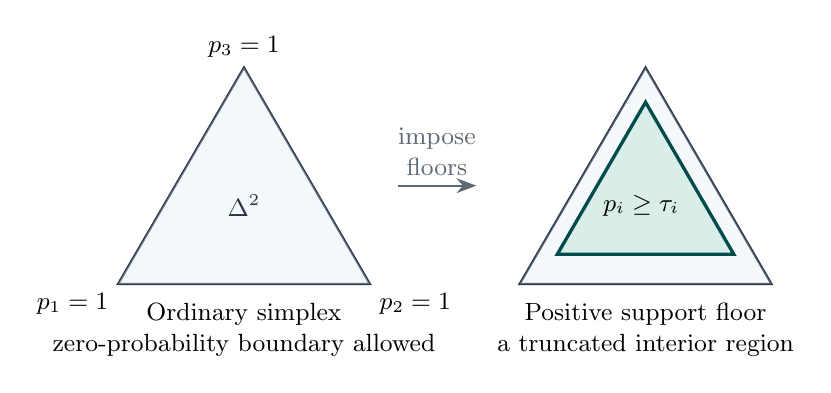
\begin{tikzpicture}[scale=1.0, every node/.style={font=\small}]
  % left simplex
  \begin{scope}[xshift=0cm]
    \coordinate (A) at (0,0); \coordinate (B) at (3.2,0); \coordinate (C) at (1.6,2.75);
    \draw[thick,slate] (A)--(B)--(C)--cycle;
    \fill[bluefill,opacity=.35] (A)--(B)--(C)--cycle;
    \node[below left] at (A) {$p_1=1$};\node[below right] at (B) {$p_2=1$};\node[above] at (C) {$p_3=1$};
    \node[align=center] at (1.6,-.58) {Ordinary simplex\\zero-probability boundary allowed};
    \node[slate] at (1.6,1.0) {$\Delta^2$};
  \end{scope}
  % right inset simplex
  \begin{scope}[xshift=5.1cm]
    \coordinate (A2) at (0,0); \coordinate (B2) at (3.2,0); \coordinate (C2) at (1.6,2.75);
    \draw[thick,slate] (A2)--(B2)--(C2)--cycle;
    \fill[bluefill,opacity=.28] (A2)--(B2)--(C2)--cycle;
    \coordinate (a) at (.48,.38); \coordinate (b) at (2.72,.38); \coordinate (c) at (1.6,2.31);
    \fill[tealfill,opacity=.95] (a)--(b)--(c)--cycle;
    \draw[very thick,teal!60!black] (a)--(b)--(c)--cycle;
    \node[below left] at (A2) {};\node[below right] at (B2) {};\node[above] at (C2) {};
    \node[align=center] at (1.6,-.58) {Positive support floor\\a truncated interior region};
    \node[align=center] at (1.6,1.0) { $p_i\geq\tau_i$ };
  \end{scope}
  \draw[-{Stealth[length=2.5mm]},thick,muted] (3.55,1.25)--(4.55,1.25) node[midway,above,align=center] {impose\\floors};
\end{tikzpicture}
\caption{Schematic geometry on a three-outcome simplex. A positive floor removes boundary regions. For general coupling polytopes the truncation can alter the face structure or make the feasible set empty; it does not automatically preserve the original toric fan.}
\label{fig:simplex}
\end{figure}

\subsection{The weakest link: slack and robustness}

For a candidate coupling $\pi$, define cellwise slack
\[
 s_{xy}(\pi)=\pi_{xy}-\tau_{xy},\qquad
 s_{\min}(\pi)=\min_{(x,y)\in D}s_{xy}(\pi),
\]
where $D$ is the set of designated cells. Positive minimum slack means every designated cell clears its floor; zero means at least one is active at the boundary; negative slack means the candidate violates the policy.

A stronger, polytope-level diagnostic asks how much additional support can be guaranteed simultaneously. With positive weights $w_k$ setting the scale of each requirement, solve
\begin{equation}\label{eq:robust}
\begin{aligned}
  \delta^\star=\max_{\pi,\delta}\quad &\delta\\
  \text{subject to}\quad&A\pi=b,\\
  &\pi_k\geq\tau_k+w_k\delta\quad(k\in D),\\
  &\pi\geq0,\quad \mathbf{1}^{\mathsf T}\pi=1.
\end{aligned}
\end{equation}
The value $\delta^\star$ is a common additional margin above the required floors, under the chosen scaling. A positive value indicates headroom; zero identifies a bottleneck; a negative optimum indicates that the floors cannot all be met. Since this is a linear program, rational inputs permit exact rational certificates in principle.

For coupled local models, the overall weakest link should not be collapsed prematurely into one scalar. Keep a typed signature such as
\[
  \Ob=(\Ob_{\mathrm{supp}},\Ob_{\mathrm{glue}},\Ob_{\mathrm{comp}},\Ob_{\mathrm{evid}}),
\]
where the components record support shortfall, failure to glue, failure to compose, and inadequate or conflicting evidence. They have different mathematical types; combining them into a single score requires an explicit normalization and decision policy.

\section{Why a presheaf: local chains without an assumed global outcome}

\subsection{The local-first principle}

A global emergent property may not exist, or may exist only after adding assumptions that the evidence does not justify. In that situation, a global model should not be the data structure's default. Instead, let each context carry its own local probability object, support policy, and evidence trail. Restriction maps describe what remains visible when moving to a smaller context. Compatibility asks whether the local objects agree on overlaps. Gluing asks whether compatible local objects come from a single global object.

This is precisely the use-case for a presheaf. For a category of contexts $\Ctx$ (often a poset ordered by inclusion), a presheaf is a contravariant functor
\[
  F:\Ctx^{\mathrm{op}}\longrightarrow\mathbf{Set}
\]
(or to a suitable category of probability spaces, constraint objects, or provenance records). A context $U$ is assigned a set $F(U)$ of admissible local descriptions; an inclusion $V\subseteq U$ induces a restriction map $\rho^U_V:F(U)\to F(V)$. Functoriality requires identity and composition of restrictions.

A presheaf does not assert that a global section exists. It gives a disciplined way to state the local data and the maps between them, and then ask whether compatible local sections glue. In an AMB measurement scenario, the familiar assignment presheaf has local sections on measurement contexts; contextuality can be expressed as a compatible family that fails to extend globally. The obstruction is meaningful precisely because local compatibility does not force a global section.

\begin{figure}[ht]
\centering
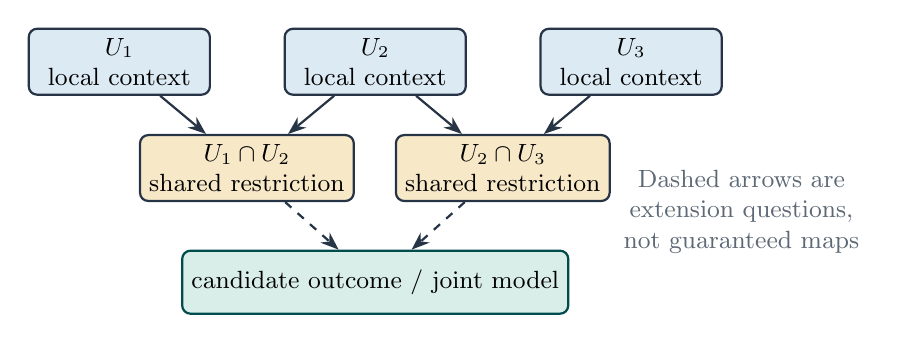
\begin{tikzpicture}[
  ctx/.style={draw=slate,rounded corners=3pt,thick,fill=bluefill,minimum width=2.3cm,minimum height=.75cm,align=center},
  outcome/.style={draw=teal!60!black,rounded corners=3pt,thick,fill=tealfill,minimum width=2.5cm,minimum height=.8cm,align=center},
  arrow/.style={-{Stealth[length=2.3mm]},thick,slate},
  every node/.style={font=\small}]
  \node[ctx] (U1) at (0,2.5) {$U_1$\\local context};
  \node[ctx] (U2) at (3.25,2.5) {$U_2$\\local context};
  \node[ctx] (U3) at (6.5,2.5) {$U_3$\\local context};
  \node[ctx,fill=amberfill] (O12) at (1.62,1.15) {$U_1\cap U_2$\\shared restriction};
  \node[ctx,fill=amberfill] (O23) at (4.87,1.15) {$U_2\cap U_3$\\shared restriction};
  \draw[arrow] (U1)--(O12);\draw[arrow] (U2)--(O12);
  \draw[arrow] (U2)--(O23);\draw[arrow] (U3)--(O23);
  \node[outcome] (Y) at (3.25,-.3) {candidate outcome / joint model};
  \draw[arrow,dashed] (O12)--(Y);
  \draw[arrow,dashed] (O23)--(Y);
  \node[align=center,text=muted] at (7.9,.6) {Dashed arrows are\\extension questions,\\not guaranteed maps};
\end{tikzpicture}
\caption{Local contexts restrict to shared overlaps. The presheaf records local descriptions and restriction maps; whether they extend to a global outcome is a separate question.}
\label{fig:presheaf}
\end{figure}

\subsection{The ``spring-leaf'' intuition, made precise}

The image of a spring leaf is useful as a design metaphor: each local segment bears a portion of the constraint load and transmits it to the next segment, while allowing local flex. The mathematical object should not be called a new standard structure without definition. We formalize it as a \emph{local constraint chain}: a path
\[
  U_0\xleftarrow{\rho_1}U_1\xleftarrow{\rho_2}\cdots
  \xleftarrow{\rho_n}U_n
\]
with local states $s_i\in F(U_i)$, restriction/transport maps between them, and a recorded support slack and obstruction at each stage. A local conclusion is carried forward only when the relevant compatibility conditions are met. When they fail, the chain records where and why it failed instead of inventing a global state.

\begin{figure}[ht]
\centering
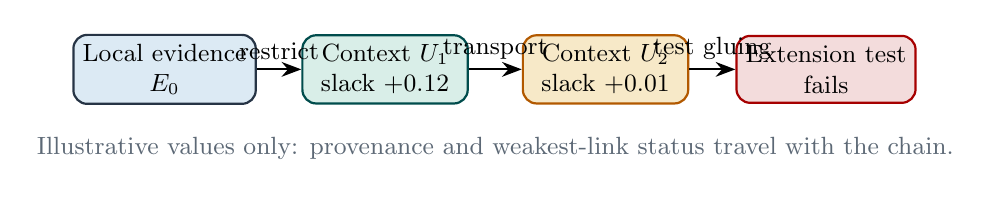
\begin{tikzpicture}[
  leaf/.style={draw=slate,rounded corners=5pt,fill=bluefill,thick,minimum width=2.1cm,minimum height=.85cm,align=center},
  good/.style={draw=teal!60!black,fill=tealfill,thick},
  weak/.style={draw=orange!70!black,fill=amberfill,thick},
  bad/.style={draw=red!65!black,fill=rosefill,thick},
  arr/.style={-{Stealth[length=2.5mm]},thick},every node/.style={font=\small}]
  \node[leaf] (a) at (0,0) {Local evidence\\$E_0$};
  \node[leaf,good] (b) at (2.8,0) {Context $U_1$\\slack $+0.12$};
  \node[leaf,weak] (c) at (5.6,0) {Context $U_2$\\slack $+0.01$};
  \node[leaf,bad] (d) at (8.4,0) {Extension test\\fails};
  \draw[arr] (a)--node[above,align=center]{restrict} (b);
  \draw[arr] (b)--node[above,align=center]{transport} (c);
  \draw[arr] (c)--node[above,align=center]{test gluing} (d);
  \node[align=center,text=muted] at (4.2,-1.0) {Illustrative values only: provenance and weakest-link status travel with the chain.};
\end{tikzpicture}
\caption{A local chain as a spring-leaf metaphor: constraints are carried stepwise, the slack can shrink, and the process can stop at an explicit obstruction without asserting a global outcome.}
\label{fig:chain}
\end{figure}

The metaphor also clarifies the difference between a \emph{pathwise} chain and a presheaf. A chain follows one route through contexts. A presheaf records all restriction maps and their compatibility, including multiple routes that may disagree. If two paths produce different transported conclusions, that disagreement can be tracked as a path-dependence or holonomy-like diagnostic; it should not automatically be identified with the AMB contextuality class or Vigneaux's information cohomology.

\section{AMB and Vigneaux: use both vocabularies without claiming a false bridge}

The attached holonomy analysis makes a crucial distinction that this proposal preserves. Abramsky--Mansfield--Barbosa (AMB) study contextuality using support sections and cohomological obstructions on a measurement cover. Vigneaux's framework studies information structures, observables, conditioning actions, and cohomological information functionals. The two frameworks emphasize different local objects and coefficient systems.

\begin{itemize}[leftmargin=2em]
  \item \textbf{AMB side:} represent a measurement scenario by its contexts and assignment presheaf. The support of each empirical model determines which local sections are permitted. A compatible family may fail to extend to a global section; the obstruction is a contextuality witness.
  \item \textbf{Vigneaux side:} represent the information structure by observables equipped with the conditioning action. Information functionals such as entropy live in that setting, and the action matters to the cohomological differential.
  \item \textbf{Proposed support ambience:} attach floors, uncertainty bands, provenance, and local obstruction records to each context. This enriches the data carried locally, but does not identify the AMB and Vigneaux coefficient systems.
\end{itemize}

In particular, the support indicator taking a positive section to $1$ and an empty section to $0$ is not additive: two positive sections can combine to a positive section. It therefore is not a morphism of abelian-group coefficient systems and cannot induce the proposed cohomology map. Nor does a holonomy cocycle of known transformations become the AMB obstruction merely because both are local. As emphasized in the supplied holonomy note, these are distinct cocycles of distinct objects. We use the two terminologies side by side and seek a richer context object, not a direct identification of their existing cohomology classes.

\subsection{A useful division of labor}

The presheaf answers: \emph{what local states exist, and how do they restrict?} The support-constrained polytope answers: \emph{which probability assignments satisfy the local constraints and floors?} The Vigneaux-style conditioning action answers: \emph{how does the information functional respond when we condition and reweight?} The AMB-style extension test answers: \emph{do compatible local support sections extend to a global assignment?} Provenance answers: \emph{which evidence and policy choices led to this result?}

These are complementary questions, not interchangeable invariants.

\section{An ambience-carrying comonad}

Let $\Ctx$ be a category of contexts and admissible restriction/transport maps. A candidate ambient record is
\[
 a=(m,\tau,\mathcal E,\mathcal G,\mathcal D),
\]
where $m$ denotes marginal/conditional constraints, $\tau$ support floors, $\mathcal E$ evidence provenance, $\mathcal G$ allowed gluing/composition rules, and $\mathcal D$ the decision policy. For a candidate space $Y$, write informally
\[
 C_a(Y)=Y\times A_a,
\]
where $A_a$ stores the applicable ambience and its history. The intent is to carry the ambient record while a candidate is restricted or transported to another context.

To turn this into a genuine comonad, one must specify natural transformations
\[
 \epsilon:C\Rightarrow\mathrm{Id},\qquad
 \delta:C\Rightarrow C^2
\]
that satisfy the counit and coassociativity laws. The intended readings are:
\begin{description}[leftmargin=2em,style=nextline]
  \item[Counit] extract the current candidate from the candidate-plus-context record;
  \item[Comultiplication] expose the context together with the nested context/history needed to explain how constraints were inherited and transformed.
\end{description}

These readings are not a proof. A product construction $Y\times A$ does not automatically define a comonad with the desired transport behavior. The category of contexts, the action on morphisms, and the maps $\epsilon,\delta$ must be specified and checked. In particular, a probability threshold cannot simply be copied through an arbitrary Markov kernel: the target event may have a different meaning or probability. The transport law must say whether floors are pushed forward, re-estimated, weakened, or retained only for corresponding events.

\begin{figure}[ht]
\centering
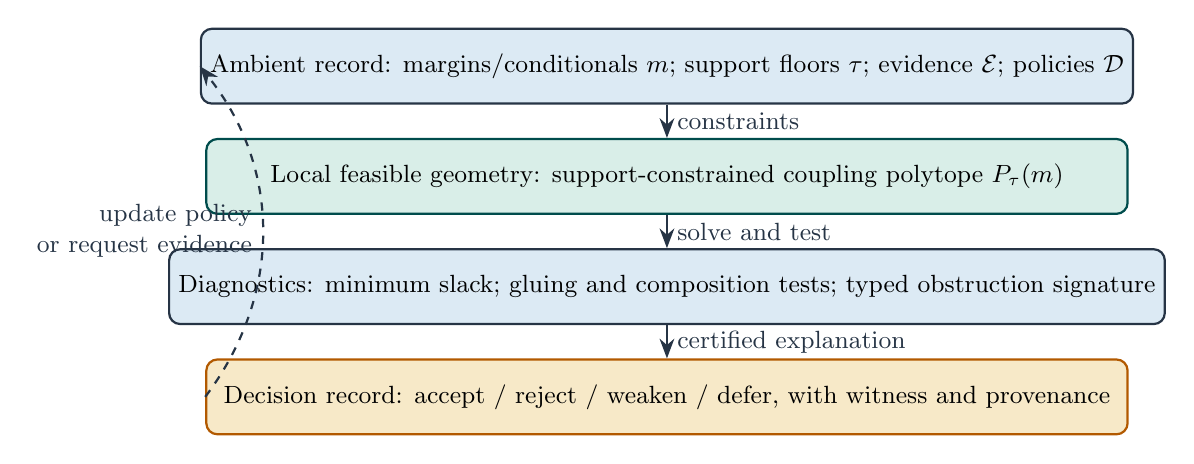
\begin{tikzpicture}[
  block/.style={draw=slate,rounded corners=4pt,thick,fill=bluefill,minimum width=11.7cm,minimum height=.95cm,align=center},
  blockg/.style={draw=teal!60!black,rounded corners=4pt,thick,fill=tealfill,minimum width=11.7cm,minimum height=.95cm,align=center},
  blocka/.style={draw=orange!70!black,rounded corners=4pt,thick,fill=amberfill,minimum width=11.7cm,minimum height=.95cm,align=center},
  arr/.style={-{Stealth[length=2.5mm]},thick,slate},every node/.style={font=\small}]
  \node[block] (amb) at (0,3.3) {Ambient record: margins/conditionals $m$; support floors $\tau$; evidence $\mathcal E$; policies $\mathcal D$};
  \node[blockg] (poly) at (0,1.9) {Local feasible geometry: support-constrained coupling polytope $P_\tau(m)$};
  \node[block] (diag) at (0,.5) {Diagnostics: minimum slack; gluing and composition tests; typed obstruction signature};
  \node[blocka] (dec) at (0,-.9) {Decision record: accept / reject / weaken / defer, with witness and provenance};
  \draw[arr] (amb)--node[right]{constraints} (poly);
  \draw[arr] (poly)--node[right]{solve and test} (diag);
  \draw[arr] (diag)--node[right]{certified explanation} (dec);
  \draw[arr,dashed,bend right=38] (dec.west) to node[left,align=right]{update policy\\or request evidence} (amb.west);
\end{tikzpicture}
\caption{Proposed architecture. The comonadic ambience layer carries context and history; the polytope and obstruction computations enforce and test the mathematical constraints. Feedback changes the ambience only through an explicit recorded update.}
\label{fig:architecture}
\end{figure}

\section{Decision provenance and typed obstruction records}

Each decision should return a record of the form
\[
 R=(d,\mathcal C_{\mathrm{active}},E,W,\Ob),
\]
where $d$ is the decision, $\mathcal C_{\mathrm{active}}$ the active constraints, $E$ the evidence provenance, $W$ a witness or certificate, and $\Ob$ the obstruction signature. For example:

\begin{center}
\begin{tabular}{>{\raggedright\arraybackslash}p{.25\linewidth}p{.64\linewidth}}
\toprule
Field & Illustrative record \\
\midrule
Decision & Reject this candidate joint distribution \\
Policy & Each designated event has probability at least $0.10$ \\
Active constraint & $\pi_{23}\geq0.10$ \\
Witness & The remaining margins force $\pi_{23}\leq0.07$ \\
Weakest link & At least $0.03$ shortfall on this event \\
Provenance & Source observations, version of the margin estimate, and policy version \\
Next action & Revise the floor, revise the margins with evidence, or defer \\
\bottomrule
\end{tabular}
\end{center}

The numbers are illustrative. For linear feasibility, a dual certificate can often identify a combination of constraints that is inconsistent. For a failed gluing problem, the witness may instead be a compatible family of local sections that has no global extension. For a path-dependent operation system, it may be non-zero holonomy. The system should retain the type of witness instead of flattening all failures into a generic ``low confidence'' score.

\section{Interaction with entropy, Fisher geometry, and toric models}

A positive floor changes the admissible region, but it does not automatically change an algebraic toric equation by replacing its right-hand side zero with a positive constant. These are different mathematical operations. The safe formulation is to retain the toric/algebraic structure where it applies and intersect the probability polytope with the linear support inequalities.

On the positive interior of a probability simplex, entropy and the Fisher metric give useful differential-geometric structure. A support floor keeps the selected coordinates away from the corresponding boundary, so it can improve regularity on the constrained region. However, truncation can change the face structure and need not preserve the original toric fan or the original interpretation of every facet. The toric realization, Fano property, and disc-potential formula must be checked separately for each new polytope/model.

For gluing, a standard example is a joint distribution of $(X,Y,Z)$ with fixed $(X,Y)$ and $(Y,Z)$ marginals. The maximum-entropy filler, when the relevant positive shared marginal is well-defined, satisfies
\[
 H(X,Y,Z)\leq H(X,Y)+H(Y,Z)-H(Y),
\]
with equality exactly when $X\perp Z\mid Y$. A support floor can exclude this maximum-entropy filler even when unconstrained gluing is possible. Thus we should track at least three separate statuses: existence of any filler, existence of a filler meeting the support policy, and entropy-optimality among the admissible fillers.

\section{A minimal experimental programme}

\begin{enumerate}[leftmargin=2em]
  \item \textbf{Three binary variables.} Fix pairwise margins for $(X,Y)$ and $(Y,Z)$. Enumerate or optimize over joint fillers and sweep a common floor $\tau$.
  \item \textbf{Record the support margin.} Compute feasibility and $\delta^\star$ from \eqref{eq:robust}; identify which cell becomes active first.
  \item \textbf{Separate obstructions.} Record ordinary gluing feasibility, support-constrained gluing feasibility, and any conditional-independence/entropy statement separately.
  \item \textbf{Vary the ambience.} Change the floor and evidence version while preserving a provenance trail. Verify that each decision can be replayed from its recorded inputs.
  \item \textbf{Test local-to-global behavior.} Use a cyclic family of contexts with overlapping variables. Store local sections in a presheaf and test whether compatible sections glue; do not assume that a single fitted corpus can witness its own inconsistency.
  \item \textbf{Test transport.} Apply deterministic maps and genuinely stochastic kernels separately. Specify how the support policy transports before asserting functoriality or comonad laws.
\end{enumerate}

\section{Claims and limits}

\paragraph{Proposed.} Support floors as ambient parameters; a presheaf of local probability/support/provenance data; weakest-link and typed-obstruction diagnostics; and a context-carrying comonadic design.

\paragraph{Mathematically immediate.} Intersecting a coupling polytope with finitely many support inequalities gives a (possibly empty) polytope. The max--min margin program is linear. Presheaves encode restriction and do not assume a global section exists.

\paragraph{Not established by this proposal.} That the proposed ambience assignment defines a comonad; that the comonad preserves support floors under arbitrary stochastic transport; that the truncated polytope inherits the original toric geometry; or that the AMB and Vigneaux cohomologies are unified. Each requires a separate definition and proof. In particular, the supplied holonomy analysis argues against a direct coefficient-system morphism between AMB support cohomology and Vigneaux's information cohomology; this proposal does not claim to overturn that result.

\section{Conclusion}

The central design choice is to make support a local, policy-dependent geometric constraint and to carry its provenance alongside the probability object. A presheaf is appropriate because the system may have meaningful local chains and outcomes without a single global emergent structure. The ``spring-leaf'' picture becomes a family of local sections connected by restriction and transport maps, with slack and obstruction witnesses carried at every step. A comonad may provide the ambient memory of how those constraints were inherited, but only after its maps and laws are made precise. This yields an auditable route from evidence through local probability geometry to a decision, with the weakest link exposed rather than hidden.

\begin{thebibliography}{9}
\bibitem{AMB}
S. Abramsky, S. Mansfield, and R. S. Barbosa,
\newblock The cohomology of non-locality and contextuality,
\newblock \emph{Electronic Proceedings in Theoretical Computer Science} 95 (2012), 1--14.

\bibitem{Vigneaux}
J.-P. Vigneaux,
\newblock \emph{Topology of Statistical Systems: A Cohomological Approach to Information Theory},
\newblock Ph.D. thesis, Universit\'e Paris Diderot, 2019.

\bibitem{BB}
P. Baudot and D. Bennequin,
\newblock The homological nature of entropy,
\newblock \emph{Entropy} 17(5) (2015), 3253--3318.

\bibitem{Vorobev}
N. N. Vorob'ev,
\newblock Consistent families of measures and their extensions,
\newblock \emph{Theory of Probability and its Applications} 7 (1962), 147--163.

\bibitem{HolonomyNote}
\newblock \emph{Holonomy obstructions for composed local operations, and why they succeed where marginal obstructions fail},
\newblock user-supplied manuscript, draft dated September 2026.
\end{thebibliography}

\end{document}
